\ifx\allfiles\undefined
\documentclass[12pt, a4paper, oneside]{ctexbook}
%\usepackage{microtype}
\usepackage{amsmath, esint,amsthm, amssymb, bm, color, framed, graphicx, imakeidx, geometry,
hyperref, mathrsfs,lipsum,fancyhdr,indentfirst,array,tabularx,float,prettyref,stmaryrd}
%文内引用
%插入书签:\label{myref:引用内容(英文字母,中文出现了编译错误)}
%引用书签:\prettyref{myref:引用内容}

\allowdisplaybreaks[4]

%简化的指令
%\renewcommand{\i}{\mathrm{i}}%虚数i
\newcommand{\di }{\text{d}}%微分
\newcommand{\pian }{\partial}%偏导数
\newcommand{\die }{\textbf{d}}%外微分
\newcommand{\fuyi }{^{-1}}%逆映射
\newcommand{\card }{\text{card}}%势
\newcommand{\R }{\mathbb{R}}%实数
\newcommand{\Z }{\mathbb{Z}}%整数
\newcommand{\RR }{$\R\ $}%实数(文本)
\newcommand{\Rn }{$\R^n\ $}%实数(文本)
\newcommand{\N }{\mathbb{N}}%自然数
\renewcommand{\S}{\mathcal{S}}%S
\newcommand{\fai }{\varphi}%常用的那个小phi
\newcommand{\e }{\vec{e}}%向量e
\newcommand{\Id }{\text{Id}}%单位元
\newcommand{\continue }{\text{连续}}%连续
\newcommand{\C }{\mathcal{C}}%连续函数类
\newcommand{\Com }{\mathbb{C}}%复数
\newcommand{\M }{\mathcal{M}}%矩阵
\newcommand{\Hess }{\text{Hess}}%Hess矩阵
\newcommand{\normmm}[1]{{\left\vert\kern-0.25ex\left\vert\kern-0.25ex\left\vert #1 
   \right\vert\kern-0.25ex\right\vert\kern-0.25ex\right\vert}}%|||v|||三个竖线的范数
%常用的文本里的字母
\newcommand{\x }{$x$}\newcommand{\xo }{$x_0$}
\newcommand{\y }{$y$}\newcommand{\yo }{$y_0$}
\newcommand{\z }{$z$}\newcommand{\zo }{$z_0$}
\newcommand{\n }{$n$}\newcommand{\f  }{$ f $}

\title{
\vspace{-2cm}
  \begin{figure}[!t]%插入题目的图片
    \centering
    
\includegraphics[width=14cm]{shulijichu-2.png}
  \end{figure}
  \vspace{-2cm}
  {\Huge{\textbf{工程师学院数学理论基础\\
Fondements des Théories Mathématiques de l'Ecole d'Ingénieur de Chimie Pékin\\
第七部分:数学应用\\
Partie VII: Applications Mathématiques
}}}
}
\author{Augustin}
\date{最后更新于:\today}
\linespread{1.5}
\makeindex

\setcounter{tocdepth}{1}%两个2说明只显示到subsection
\setcounter{secnumdepth}{2}

%\def\allfiles{}
\begin{document}
\newrefformat{myref}{第\ref{#1} 节}
\vspace{-3cm}
\maketitle
\tableofcontents
\else
\part{数学应用\\ Applications Mathématiques}
\fi
%开始本部分正文
事先声明,物理是我最不会的东西.写得烂就别怪我了.
\chapter{误差与不确定度\\Erreurs et Incertitudes}
\section{全微分误差估计}
\chapter{量纲分析\\ Analyse Quantitative}
\chapter{概率论入门\\Introduction: La Probabilité}
\chapter{简单数学模型\\ Modèle Mathématique Simple}  
\chapter{离散优化模型\\ Modèles d'Optimisation Discrets} 
\chapter{连续优化模型\\ Modèle d'Optimisation Continue} 


\chapter{数学物理方程\\ Équations Mathématiques Physiques}%记得放到后面去!放前面仅仅是为了方便写.
\section{波动方程 Équation des Ondes}
\subsection{Introduction}
\subsubsection{波 Onde}
波是干扰在介质中的传播,没有任何物质的相对位移.这种传播允许信息和/或能量的传输.
这种波的特点是一个标量或矢量场,这个场的空间和时间依赖性是由偏微分方程耦合的.
波的传播可以是机械的,也可以是电磁的.机械波需要介质,而电磁波可以在真空中传播.
\\
\indent
Une onde est une propagation d'une perturbation dans un milieu sans déplacement relatif de matière.
Cette propagation permet la transmission d'information et/ou d'énergie.
Cette onde est caractérisée par un champ scalaire ou vectoriel.
Les dépendances spatiales et temporelles sont couplées par des équations aux dérivées partielles.
La propagation d'une onde peut être mécanique ou électromagnétique.
\subsubsection{传播方程 Équation de propagation}

\subsubsection{正弦信号波 signal sinusoïdal}
正弦信号波的表达式为:
$$
  s(t)=A\cos(\omega t+\varphi)
$$
其中$A$为振幅(amplitude), $\omega$为角频率(pulsation), $\varphi$为初相位(phase a l'origine).
\subsubsection{波的平均值 valeur moyenne d'une onde}
波的平均值为:
$$
  S_{moy}=<s>=\frac{1}{T}\int_{0}^{T}s(t)\,\mathrm{d}t
$$
其中$T$为波的周期.
\subsubsection{波的均方根值/有效值 valeur efficace d'une onde}
波的均方根值为:
$$
  S_{eff}=\sqrt{<s^2>}=\sqrt{\frac{1}{T}\int_{0}^{T}s^2(t)\,\mathrm{d}t}
$$

\subsubsection{Parseval定理 Théorème de Parseval}
对于周期为$T$的周期信号$s(t)$,有:
$$
  \frac{1}{T}\int_{0}^{T}s^2(t)\,\mathrm{d}t=\frac{1}{2}\sum_{n=-\infty}^{+\infty}|c_n|^2
$$
其中$c_n$为信号$s(t)$的Fourier系数.
该定理说明了信号的均方根值等于其Fourier系数的模的平方的一半.其意义为:信号的均方根值等于其频谱的均方根值.
\subsubsection{信号的复数表示 Notation complexe d'un signal}
信号$s(t)=A\cos(\omega t+\varphi)$可以表示为:
$$
  \underline{s(t)}=Ae^{j(\omega t+\varphi)}=\underline{A}e^{j\omega t}
$$
其中$e^{j(\omega t+\varphi)}$为复指数信号.
\subsubsection{Fresnel图 Representation de Fresnel}
Fresnel图是一个复平面,其横轴为实部,纵轴为虚部.
对于两个信号的叠加,其Fresnel图为两个信号的Fresnel图的叠加,也即向量的叠加.
\subsection{弦的横向振动 Vibration Transversale des Cordes}
考虑一根绷紧的柔软均匀的轻弦$l$,其线密度为$\rho$.
弦受到一个激发,使其在一个平面内小幅度振动.
取平衡位置为\x 轴,弦位于在区间$[0,l]$上.
定义函数$u(x,t)$为弦上一点在$t$时刻的位移:
$$
  u:(0,l)\times \R\rightarrow \R
$$
$$
  (x,t)\mapsto u(x,t)
$$
分析点\x 与$x+\Delta x$间的弦的受力情况:\\

设$t$时刻弦上\x 点的切线与\x 轴正方向夹角为$\theta(x,t)$.在$t_0$时刻对任意一点\xo,有:
$$
  \tan\theta(x_0,t_0)=\frac{\pian u(x_0,t_0)}{\pian x}
$$

设弦收到的拉力为:
$$
\vec{T}(x,t)=T(x,t)\cos\theta(x,t)\e_x+T(x,t)\sin\theta(x,t)\e_u
$$
\textbf{PFD:}
$$
  \vec{T}(x,t)+\vec{T}(x+\Delta x,t)=\rho \Delta x \vec{a}
$$
弦只在$u$方向振动,则$a\e_x=0$, $\vec{a}=a\e_u=\frac{\pian^2 u}{\pian x^2}$,则有:
$$
  T(x+\Delta x,t)\cos\theta(x+\Delta x,t)-T(x,t)\cos\theta(x,t)=0
$$
$$
  T(x+\Delta x,t)\sin\theta(x+\Delta x,t)-T(x,t)\sin\theta(x,t)=\rho\Delta x\frac{\pian^2 u(x,t)}{\pian t^2}
$$

由于微小振动的近似$\frac{\pian u}{\pian x}\ll 1$,则可以认为$\sin\theta =\tan\theta=\frac{\pian u}{\pian x}$,
$\cos\theta=1$,故$T(x+\Delta x,t)=T(x,t)=T(t)$,即绳子各点的张力相等.又弦长不变,由Hooke定律得$\frac{\di T}{\di t}=0$,$T$为常数.
此时方程化简为:
$$
  \rho\Delta x\frac{\pian^2 u(x,t)}{\pian t^2}=T(\frac{\pian u(x+\Delta x,t)}{\pian x}-\frac{\pian u(x,t)}{\pian x})
$$
则有
$$
\rho\frac{\pian^2 u(x,t)}{\pian t^2}=T\frac{(\frac{\pian u(x+\Delta x,t)}{\pian x}-\frac{\pian u(x,t)}{\pian x})}{\Delta x}\xrightarrow{\Delta x\rightarrow 0}T\frac{\pian^2 u}{\pian x^2}
$$
即
$$ 
  \rho\frac{\pian^2 u}{\pian t^2}=T\frac{\pian^2 u}{\pian x^2}
$$
该方程称为弦的自由振动方程.振动沿\x 方向传播,而振动方向与传播方向垂直,该类振动称为横波振动(onde transversale).
\subsection{杆的纵向振动(连续模型) Vibration longitudinale des barres(modèle continu)}
\subsubsection{Young氏模量 Module de Young} 
Young氏模量是一个材料的弹性性质,定义为:
$$
  E=\frac{\sigma}{\epsilon}
$$
其中$\sigma=\frac{F}{S}$为应力,即单位面积的截面上受到的力,单位为$Pa$. 
$\epsilon=\frac{\Delta L}{L}$为应变,即受理后物体的形变比例,无单位.
也因此Hoooke定律可以写为:
$$
  \sigma=E\epsilon
$$
\subsection{杆的纵向振动(离散模型) Vibration longitudinale des barres(modèle discret)}
\section{d'Alembert方程的渐进解 Solutions progressives de l'équation de d'Alembert}
\subsubsection{化简}
一维d'Alembert方程:
$$
  \frac{\pian^2 u}{\pian t^2}=c^2\frac{\pian^2 u}{\pian x^2}
$$
令$\xi=x-ct,\eta=x+ct$,则有:
$$
  \frac{\pian u}{\pian x}=\frac{\pian u}{\pian \xi}\frac{\pian \xi}{\pian x}+\frac{\pian u}{\pian \eta}\frac{\pian \eta}{\pian x}=\frac{\pian u}{\pian \xi}+\frac{\pian u}{\pian \eta}
$$
$$
  \frac{\pian^2 u}{\pian x^2}=\frac{\pian^2 u}{\pian \xi^2}\frac{\pian \xi}{\pian x}+\frac{\pian^2 u}{\pian \eta^2}\frac{\pian \eta}{\pian x}=\frac{\pian^2 u}{\pian \xi^2}+\frac{\pian^2 u}{\pian \eta^2}
$$
$$
  \frac{\pian u}{\pian t}=\frac{\pian u}{\pian \xi}\frac{\pian \xi}{\pian t}+\frac{\pian u}{\pian \eta}\frac{\pian \eta}{\pian t}=c\frac{\pian u}{\pian \xi}-c\frac{\pian u}{\pian \eta}
$$
$$
  \frac{\pian^2 u}{\pian t^2}=\frac{\pian^2 u}{\pian \xi^2}\frac{\pian \xi}{\pian t}+\frac{\pian^2 u}{\pian \eta^2}\frac{\pian \eta}{\pian t}=c^2\frac{\pian^2 u}{\pian \xi^2}-c^2\frac{\pian^2 u}{\pian \eta^2}
$$
代入原方程,得:
$$
  \frac{\pian^2 u}{\pian \xi^2}-\frac{\pian^2 u}{\pian \eta^2}=0
$$
也即方程可化简为两个单独的函数,分别为$\xi$和$\eta$的函数.此时,方程的解为:
$$
  u(\xi,\eta)=f(\xi)+g(\eta)
$$
也即:
$$
  s(x,t)=f(x-ct)+g(x+ct)
$$
由于$\xi=x-ct,\eta=x+ct$,因此$\xi$和$\eta$分别表示了$x$在$t$时间内向左和向右传播的距离.因此,函数$f$和$g$分别表示了$x$在$t$时间内向左和向右传播的距离上的振动情况.因此,函数$s$表示了$x$在$t$时间内向左和向右传播的距离上的振动情况的叠加.
\subsubsection{Exemple}
\begin{enumerate}
  \item $f(x)=\sin x,g(x)=\cos x$,则有:
  $$
    s(x,t)=\sin(x-ct)+\cos(x+ct)
  $$
  \item $f(x)=\sin x,g(x)=\sin x$,则有:
  $$
    s(x,t)=\sin(x-ct)+\sin(x+ct)
  $$
  \item $f(x)=\sin x,g(x)=\sin x$,则有:
  $$
    s(x,t)=\sin(x-ct)+\sin(x+ct)
  $$
\end{enumerate}
\subsection{Onde progressive sinusoïdal (dim=1) }
方程的形式为:
$$
s(x,t)=A\cos(\omega t-kx+\phi)
$$
其中,振幅$A$为正弦波的最大值,
角频率$\omega$为正弦波的周期,
波数(vecteur d'onde)$k$为正弦波的波长,
相位$\phi$为正弦波的初始相位.
\subsubsection{Remarque:relation de dispersion}
\begin{enumerate}
  \item $k=\frac{2\pi}{\lambda}$
  \item $k^2\omega^2=c^2$
  \item $\omega=2\pi f$
  \item $v=\frac{\omega}{k}=\frac{\lambda}{T}=\lambda f$(vitesse de phase)
\end{enumerate}
对于$k>0$,即$-k<0$,波的传播方向为$+\e_x$;
对于$k<0$,即$-k>0$,波的传播方向为$-\e_x$.
\subsection{波的干涉 Interférence entre deux ondes}
\subsubsection{相长干涉 Interférence constructive}
两个波源$S_1,\,S_2$在点$M$处的相位差为:
$$
\Delta \varphi=\frac{2\pi}{\lambda}(r_2-r_1)
$$
其中$r_1=S_1M$, $r_2=S_2M$.
当$\Delta \varphi=2k\pi$,即$r_2-r_1=k\lambda$时,两个波源$S_1,\,S_2$在点$M$处的相位差为$2k\pi$,此时两个波源$S_1,\,S_2$在点$M$处的波的振幅叠加,此时为相长干涉.
\subsubsection{相消干涉 Interférence destructive}
当$\Delta \varphi=(2k+1)\pi$,即$r_2-r_1=(2k+1)\frac{\lambda}{2}$时,两个波源$S_1,\,S_2$在点$M$处的相位差为$(2k+1)\pi$,此时两个波源$S_1,\,S_2$在点$M$处的波的振幅叠加,此时为相消干涉.

\subsubsection{différence de marche}
对于两个同步的波源$S_1,\,S_2$在点$M$处的速率差为:
$$
\delta=r_2-r_1
$$
其中$r_1=S_1M$, $r_2=S_2M$.相位差为:
$$
\Delta \varphi=\frac{2\pi}{\lambda}\delta
$$
\subsubsection{干涉条纹}
干涉条纹为相长干涉和相消干涉的叠加.
干涉条纹的间距为:
$$
\delta=\frac{\lambda}{2}\frac{D}{d}
$$
其中$\lambda$为波长,
$D$为两个波源$S_1,\,S_2$到屏幕的距离,
$d$为两个波源$S_1,\,S_2$的距离.


干涉条纹的宽度为:
$$
\delta=\frac{\lambda}{2}\frac{D}{d}
$$

\subsection{波的衍射 Diffraction d'une onde}
\subsubsection{波的衍射条件}
波的衍射条件为:
$$
a\sin\theta=n\lambda
$$
其中$a$为衍射孔的宽度,
$\theta$为衍射角,
$n$为衍射级数,
$\lambda$为波长.
\subsection{驻波 Onde stationnaire}
$$
s(x,t)=f(t)\cdot g(x)
$$
谐驻波为:
$$
s(x,t)=A\cos(\omega t+\varphi)cos(kx+\psi)
$$







\section{热方程}
\subsection{Fourier定律}
Fourier定律是传人的基本定律,描述了热传导过程.设温度函数$u$为温度函数:
$$
  u:\R^3\times \R\rightarrow \R^+
$$
$$
  (x,y,z,t)\mapsto T
$$
此时定义方向向量$v\in\R^3$,称该方向的热流密度(热通量)$q_v$为温度$T$在该方向上的导数乘上系数$k$:
$$
  q_v=-k\frac{\pian u}{\pian v}
$$
其中,负号说明温度由高向低传递,$k$称为热导率,与传热介质有关.温度变化不大时$k$与$T$无关.对于各向同性的三维介质传热,$k$与热流方向和位置都无关,则热通量表示为:
$$
  q_x=-k\frac{\pian u}{\pian x},\,q_y=-k\frac{\pian u}{\pian y},\,q_y=-k\frac{\pian u}{\pian y}
$$
也即:
$$
  q=-k\nabla u(x,y,z,t)
$$
该式称为Fourier定律.
\subsubsection{Proposition}
对于各向异性的三维介质传热,$k$变成一个$3\times 3$矩阵$K$,Fourier定律写成:
$$
q=-K\cdot \nabla u
$$
\subsection{连续性方程}
考虑一个$\Delta x\times \Delta y\times \Delta z$的各向同性的长方体在$\Delta t$时间内$x$方向净流入(流入-流出)的热量:
$$
  (q_{x,x_0}-q_{x,x_0+\Delta x})\Delta y\Delta z \Delta t=(-\frac{\pian q_x(x_0)}{\pian x}\Delta x )\Delta y \Delta z \Delta t
$$
$y,z$方向同理.设该长方体内不凭空产生或消耗热量,则净积累的热量全部用于升高物体的温度.设体密度$\rho$,比热容$c$,依据能量守恒得到:
$$
  -\nabla \cdot q \Delta x\Delta y \Delta z \Delta t=\rho \Delta x\Delta y \Delta z\cdot c\cdot \Delta T
$$
也即:
$$
  \frac{\pian \rho c u}{\pian t}+\nabla \cdot q=0
$$
该式称连续性方程.
带入Fourier定律得到:
$$
  \frac{\pian \rho c u}{\pian t}-\nabla \cdot (k\nabla u)=0
$$
特别地,在一般情况下,$k,c,\rho$都是常数.定义热扩散效率或温度传导率$\kappa =\frac{k}{\rho c}$,
则有:
$$
  \frac{\pian u}{\pian t}-\kappa\nabla^2 u=0
$$
\subsubsection{Proposition}
若长方体内有热量的产生或消耗(如发生化学反应),定义表示单位体积内单位时间中热量变化的函数$F$:
$$
  F:\R^3\times \R\rightarrow \R
$$
$$
  (x,y,z,t)\mapsto q_r
$$
记$f=\frac{F}{\rho c}$,则各向同性的连续性方程表示为:
$$
  \frac{\pian u}{\pian t}-\kappa\nabla^2 u=\frac{F}{\rho c}=f
$$
\subsubsection{Proposition}
一个更一般的情况,各向异性的空间中的有源热场的连续性方程为:
$$
  \frac{\pian \rho c u}{\pian t}-\nabla \cdot (K\cdot \nabla u)=F(x,y,z,t)
$$
\section{稳态方程}
在一定条件下,物体的温度达到稳态,也即$\frac{\pian u}{\pian t}=0$,则温度场满足Poisson方程
$$
  \nabla^2u=-\frac{f}{\kappa}
$$
若无热源场$f=0$则满足Laplace方程
$$
  \nabla^2=0
$$

电场内电势$u$满足的Poisson方程:
$$
  \nabla^2u=-\frac{\rho }{\varepsilon_0}
$$

齐次波动方程
$$
    \frac{\pian^2 u}{\pian t^2}-a^2\nabla^2 u=0
$$
中$u(x,t,z,t)$随时间周期性变化,频率为$\omega$
$$
  u(x,y,z,t)=v(w,y,z)e^{j\omega t}
$$
则有Helmholtz方程:
$$
  \nabla^2v(x,y,z)+k^2v(x,y,z)=0
$$


这些说明这三个方程的稳态方程有类似的性质.
波动方程属于双曲方程,热方程属于抛物方程,其对应的Poisson方程和Laplace方程属于椭圆方程.
\section{定解条件}
\subsection{波动方程定解}
\subsection{热方程定解}




\chapter{对称群与分子对称性\\ Groupe Symétrique et Symétrie Moléculaire}
\begin{figure}[H]%插入题目的图片
  \centering
  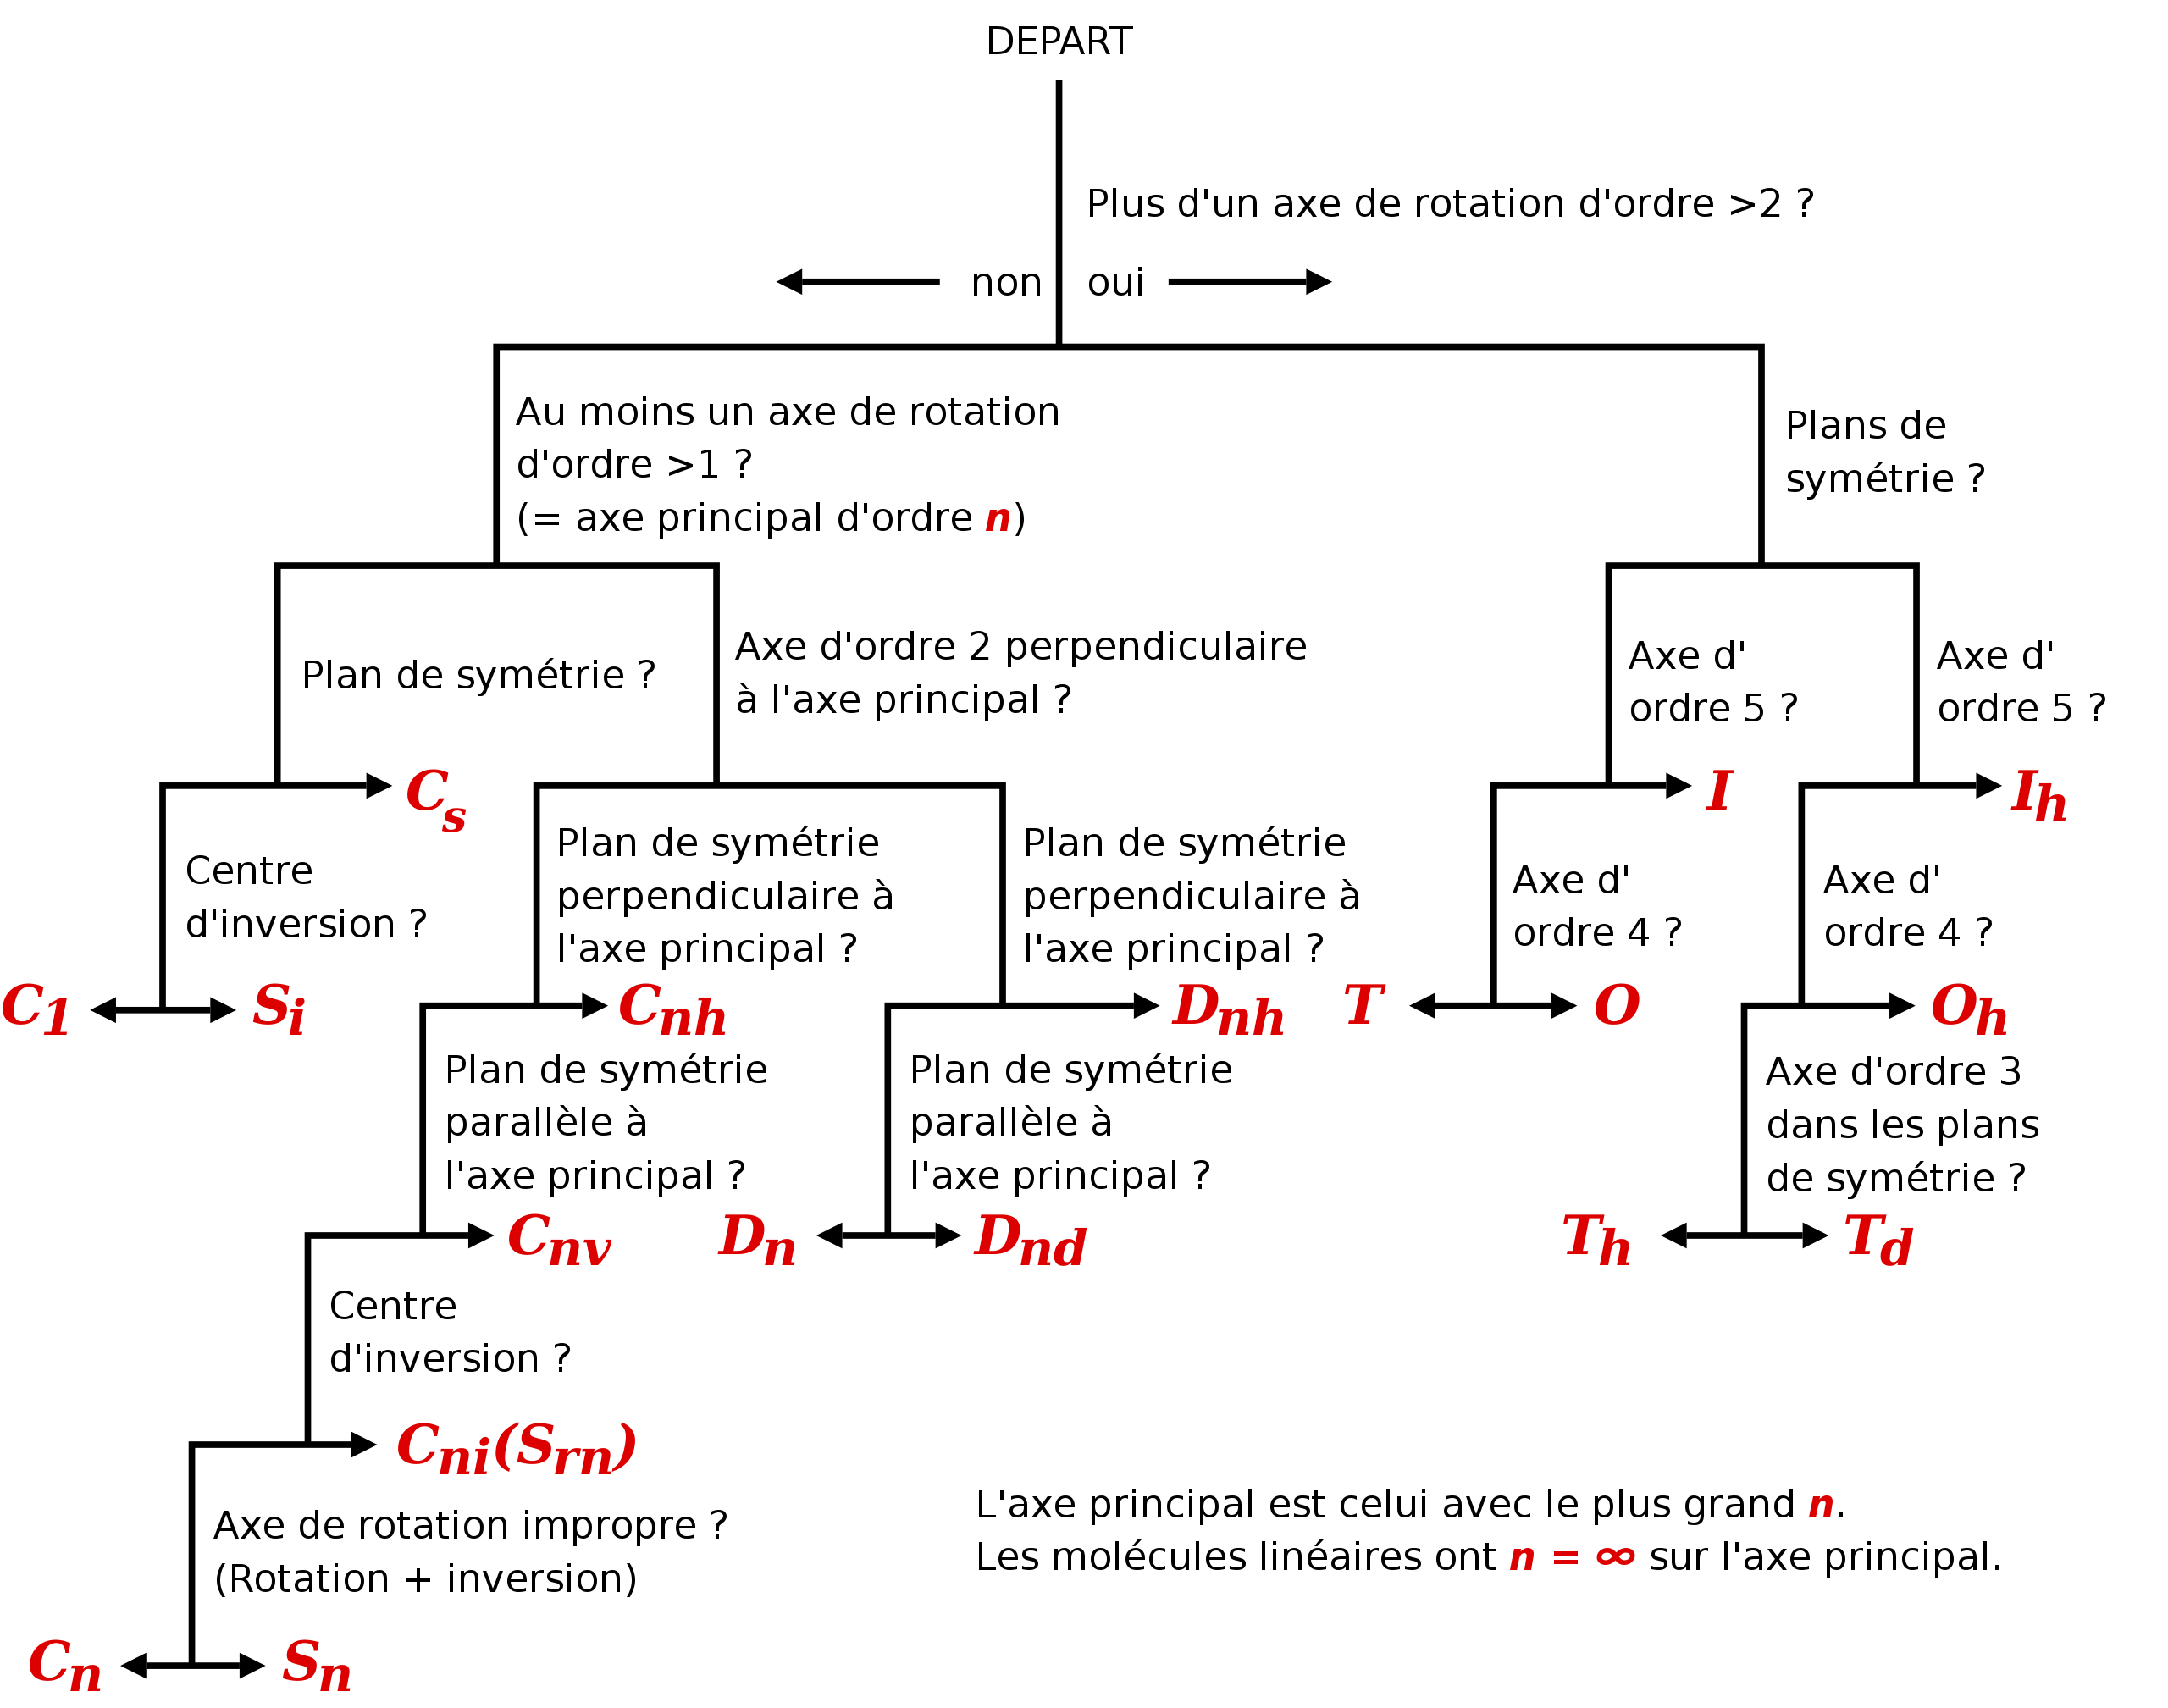
\includegraphics[scale=0.15]{groupe_chimie.png}
  \caption{群论与化学(图片源自法语wiki)}
  \label{myref:groupechimie}
\end{figure}
\section{分子对称性和对称群}
\section{群的表示}
\section{对称性匹配的线性组合}
\section{分子轨道理论}
\section{配体场理论}
\chapter{概率与位势\\ Probabilités et potentiels}  
\chapter{场论\\ Théorie des Champs} 
\chapter{电磁场\\Champs Électromagnétiques}
\chapter{引力场\\ Champ Gravitationnel}
\chapter{流体场\\Champs de Fluides}
  \section{理想流体}
  \section{实际流体}
  \section{层流与湍流}
  \section{流体边界层}








\ifx\allfiles\undefined
\end{document}
\fi